% !TeX root = ../../Skript.tex
\cohead{\Large\textbf{Ableitung trig. Funktionen}}
\fakesubsection{Ableitung trigonometrischer Funktionen}
Gegeben ist das Schaubild der Funktion \(f(x)=\sinn{x}\). Skizziere das Schaubild der Ableitung.

\begin{minipage}{\textwidth}
	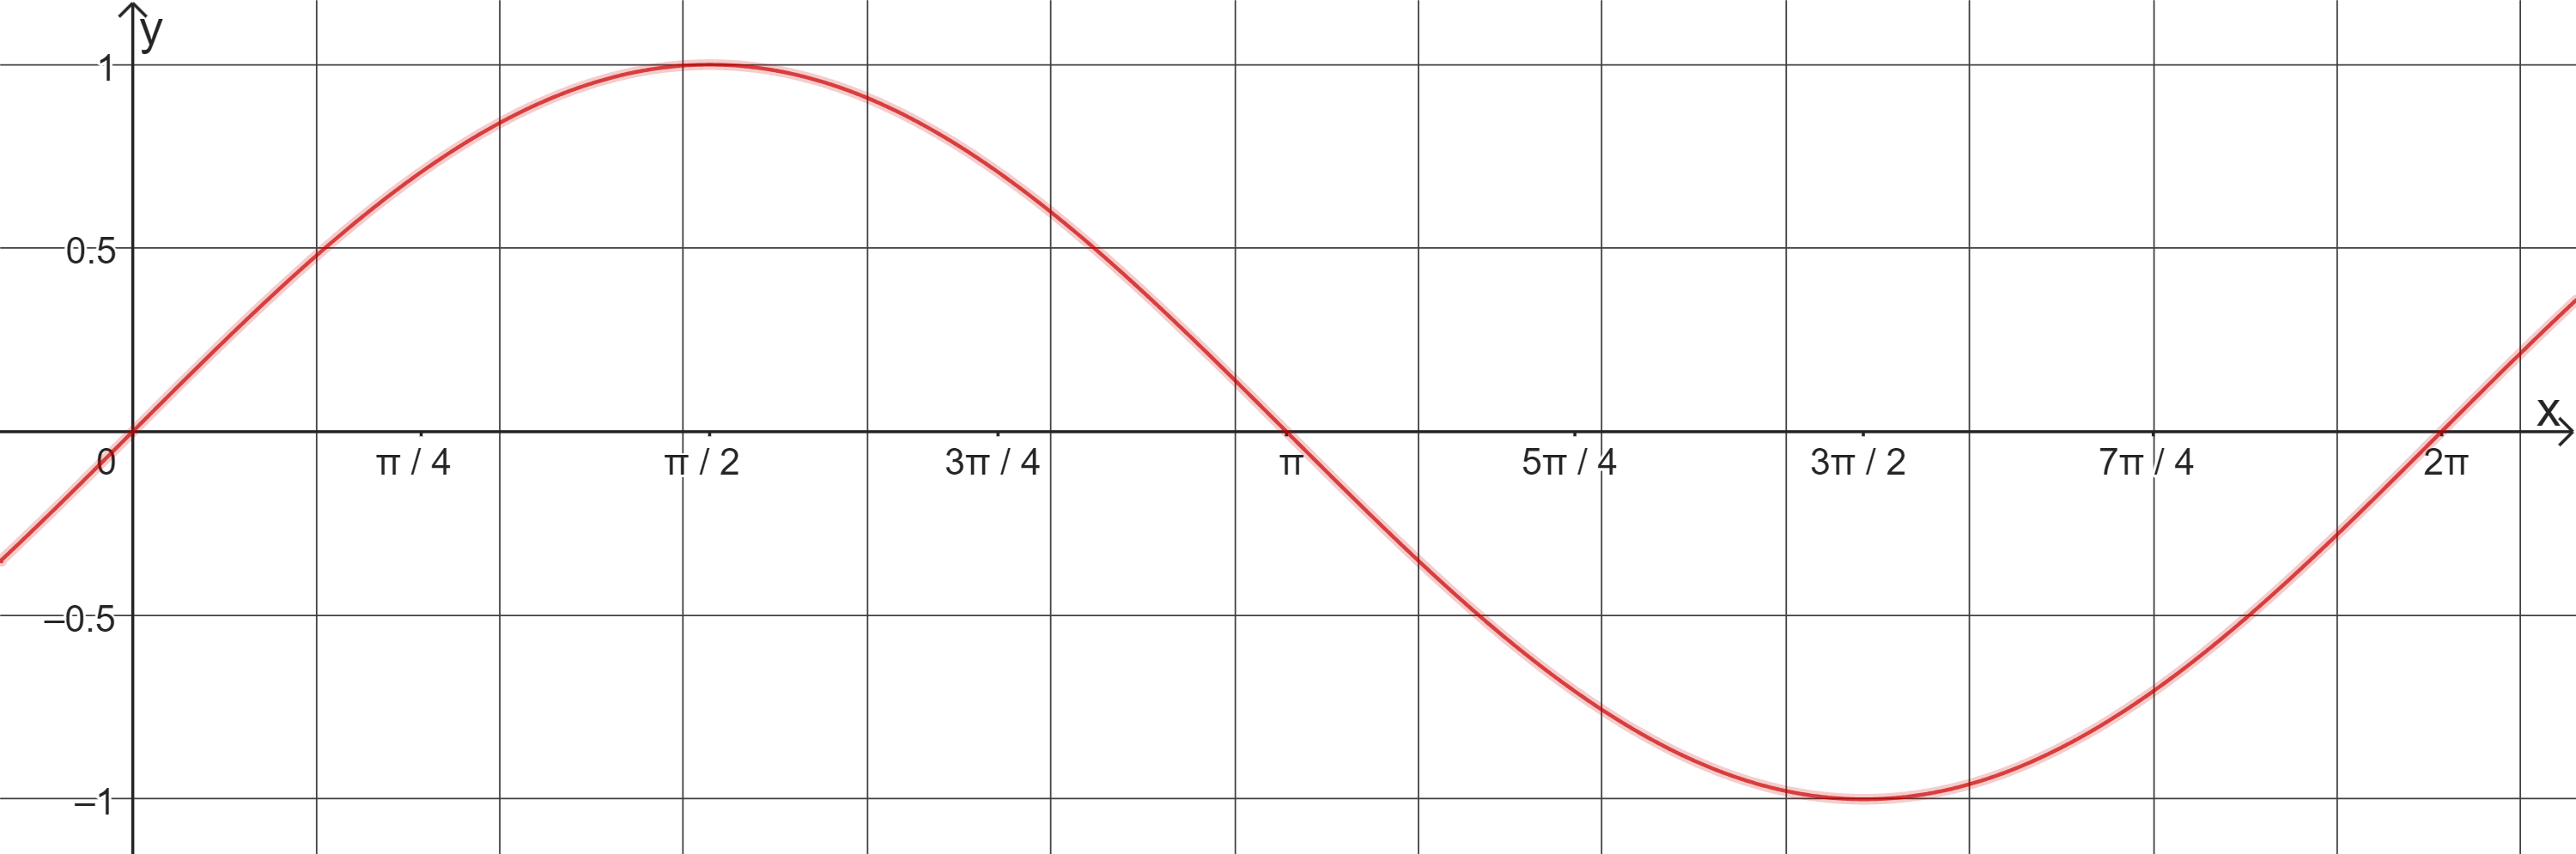
\includegraphics[width=\linewidth]{\trigonometrie/pics/AbleitungSinus.png}
\end{minipage}%

\medskip

\begin{minipage}{\textwidth}
	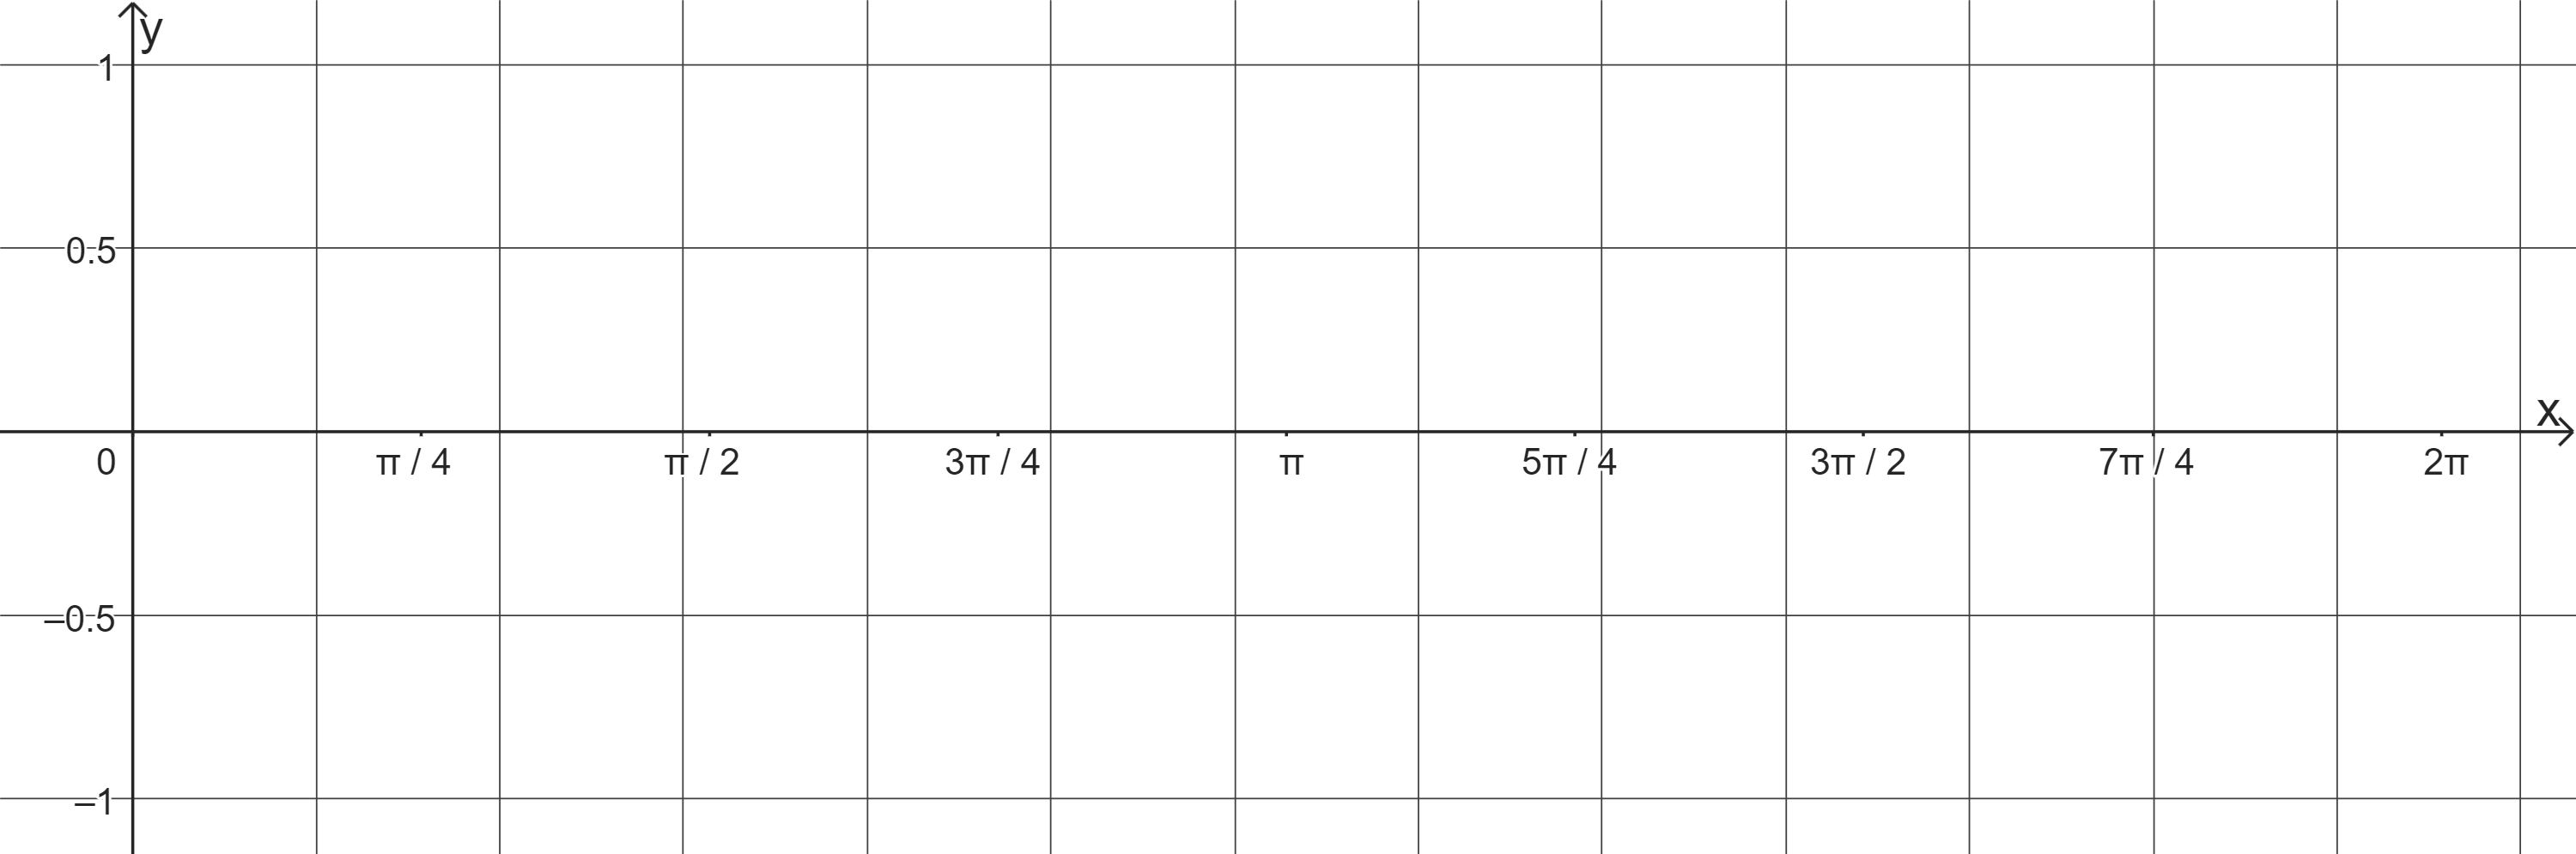
\includegraphics[width=\linewidth]{\trigonometrie/pics/AbleitungEmpty.png}
\end{minipage}%

\vspace{\baselineskip}

Gegeben ist das Schaubild der Funktion \(f(x)=\coss{x}\). Skizziere das Schaubild der Ableitung.

\begin{minipage}{\textwidth}
	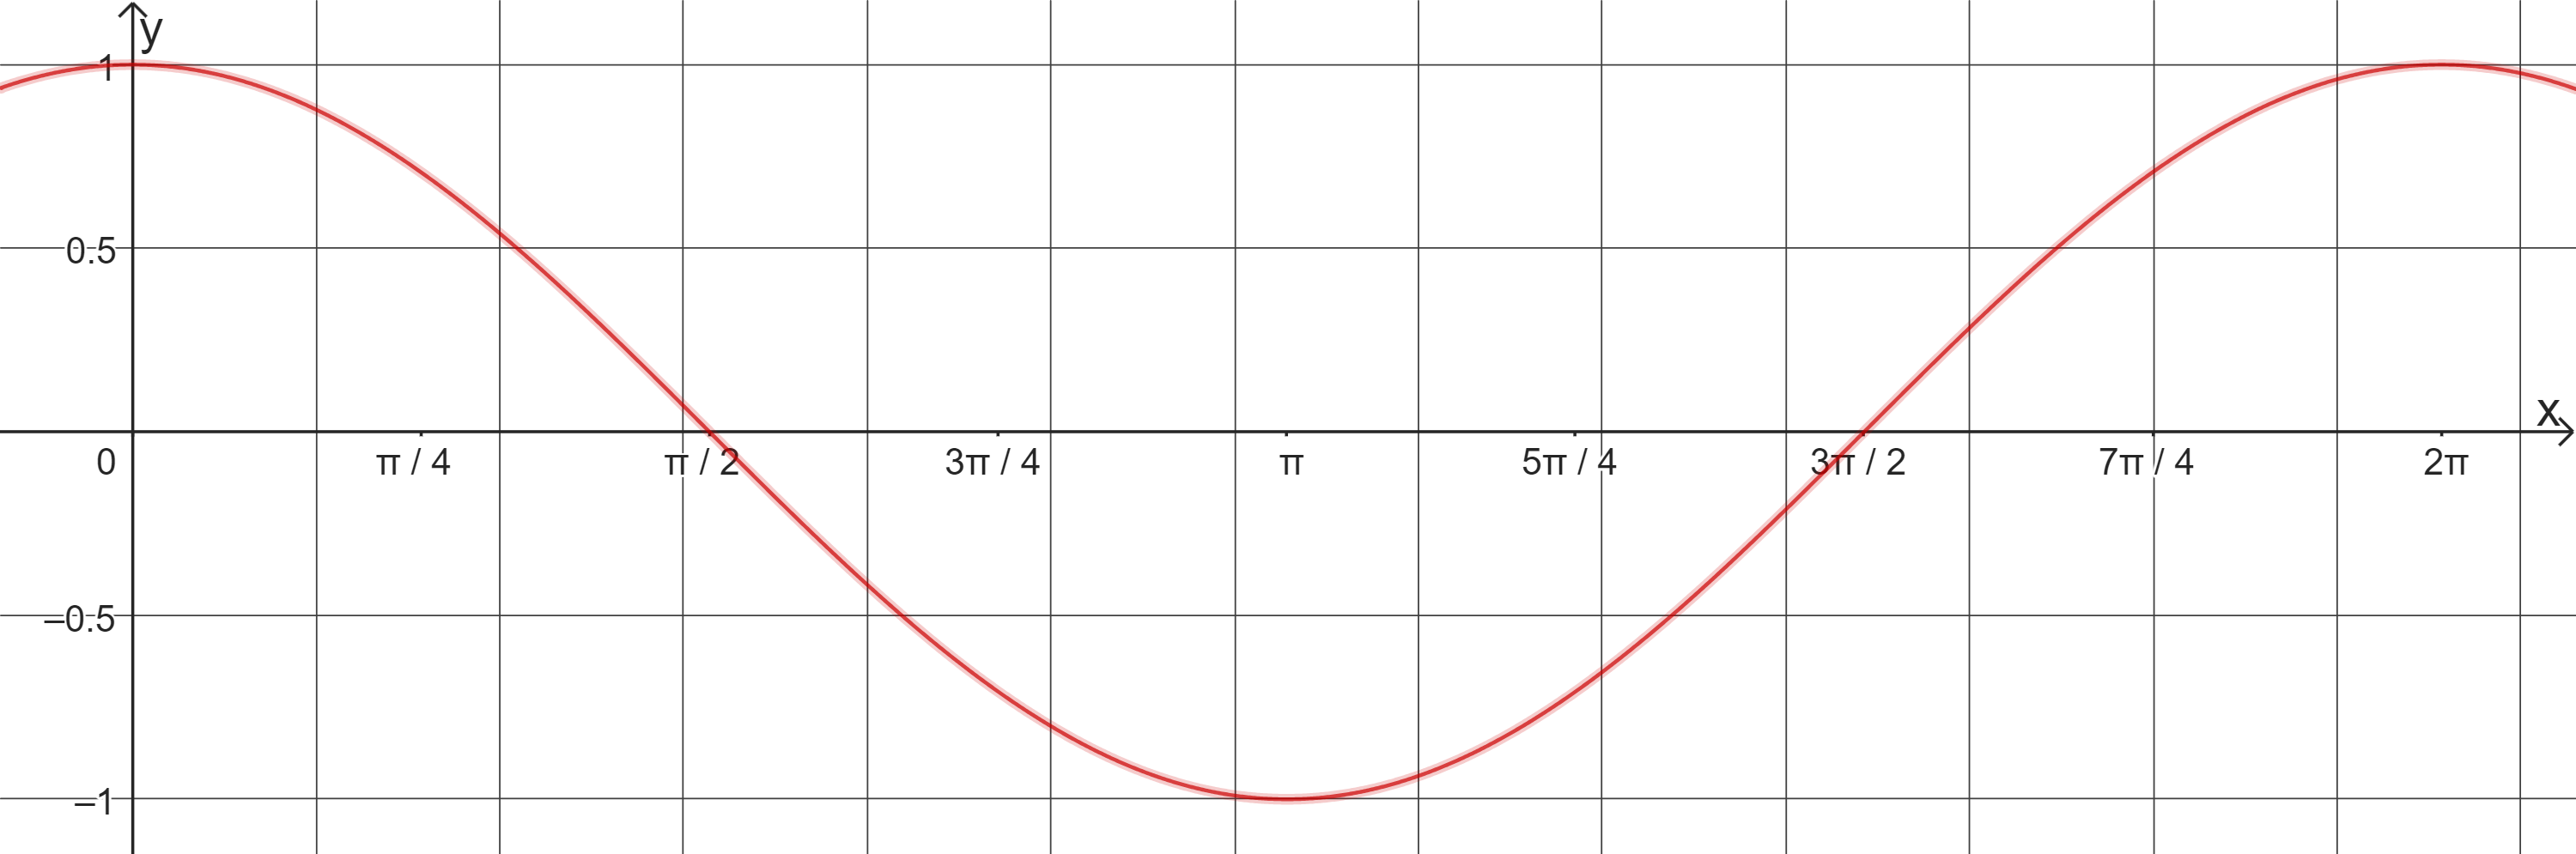
\includegraphics[width=\linewidth]{\trigonometrie/pics/AbleitungCosinus.png}
\end{minipage}%

\medskip

\begin{minipage}{\textwidth}
	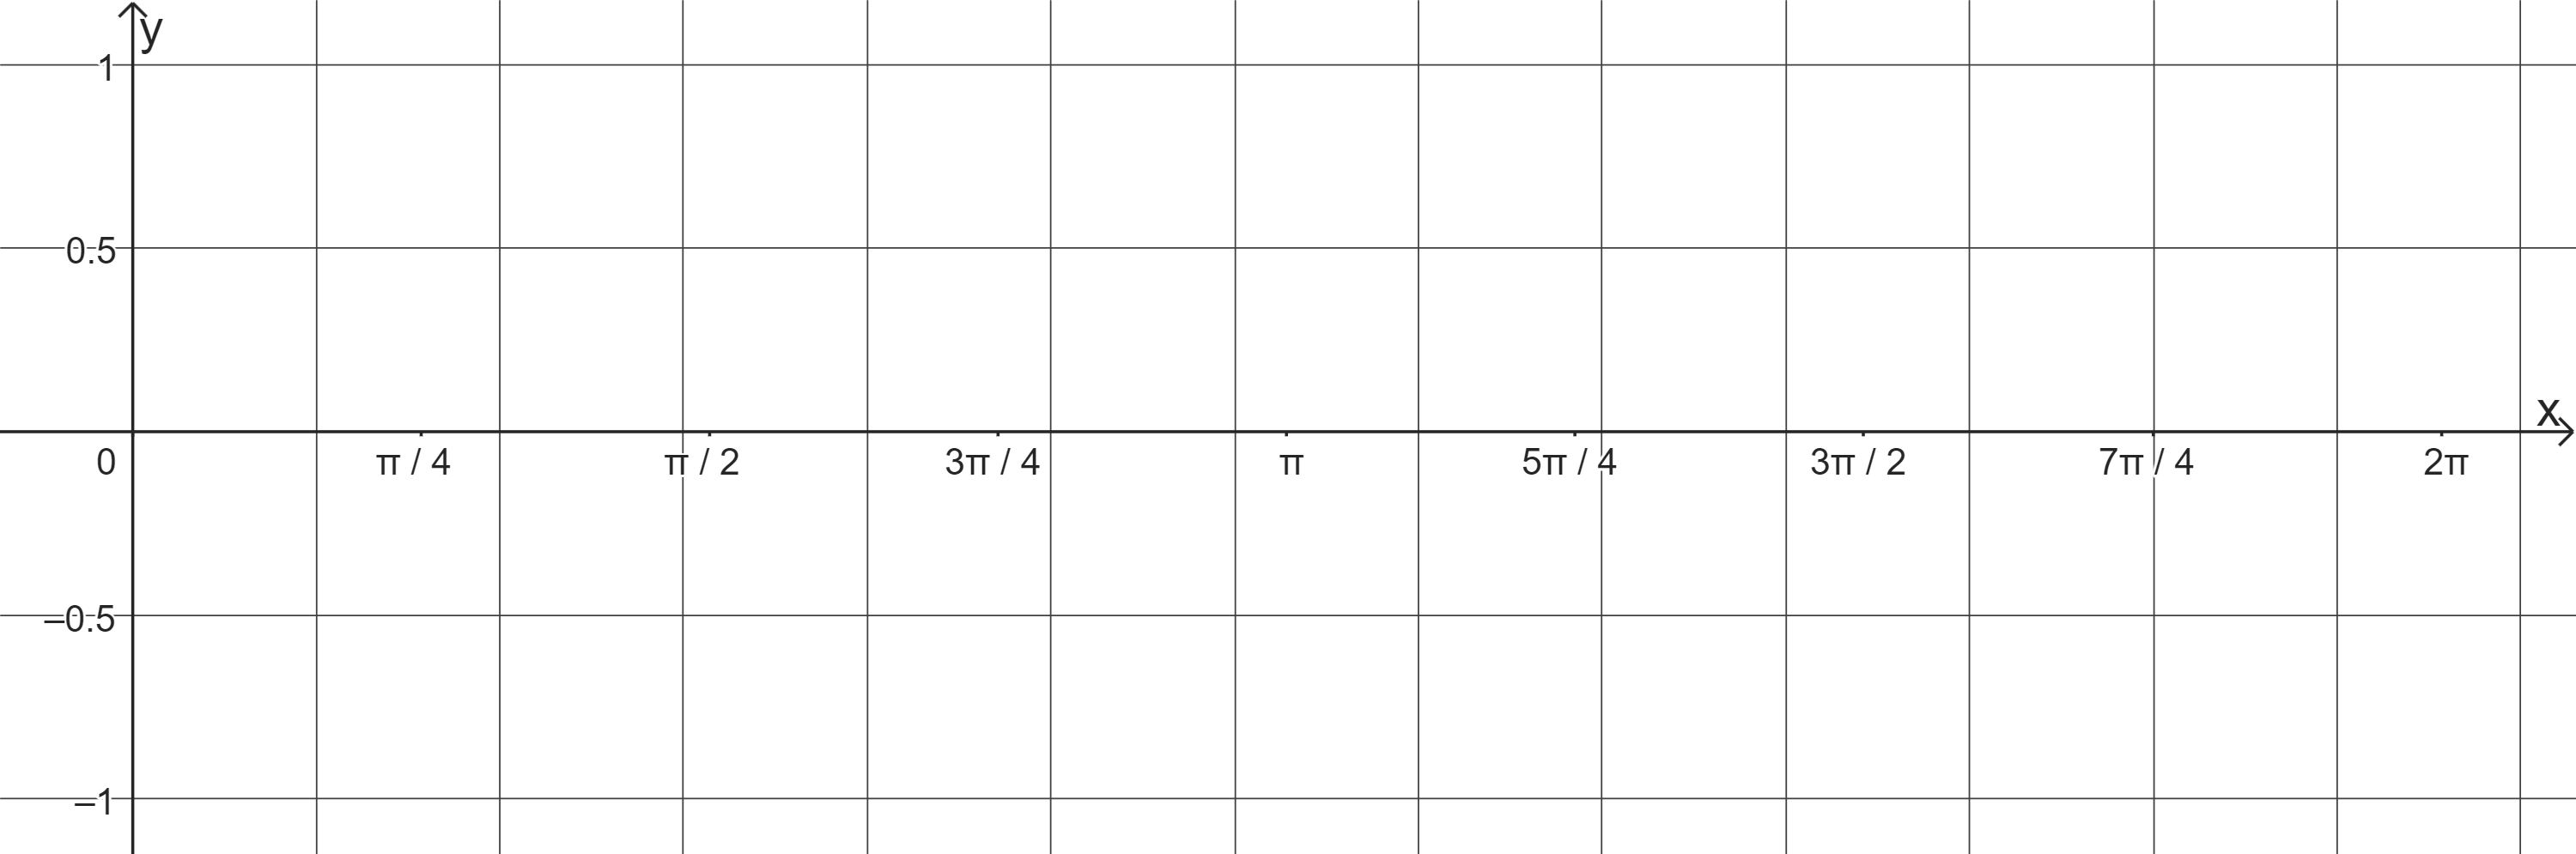
\includegraphics[width=\linewidth]{\trigonometrie/pics/AbleitungEmpty.png}
\end{minipage}%

\newpage
\iftoggle{qrcode}{\setlength{\qrheight}{2.5cm}}{\setlength{\qrheight}{0cm}}%
\newlength{\trigoAbl}%
\setlength{\trigoAbl}{\linewidth-\qrheight}%
\begin{minipage}{\linewidth}
    \adjustbox{valign=t, padding =0ex 0ex 0ex 0ex}{\begin{tcolorbox}[width=\trigoAbl]
            \textbf{Ableitungsregeln für Sinus und Cosinus}
            \begin{align*}
                f(x)&=a\cdot\sinn{bx}&g(x)&=a\cdot\coss{bx}\\
                \textcolor{loestc}{f'(x)}&\textcolor{loestc}{\;=a\cdot b\cdot\coss{bx}}&\textcolor{loestc}{g'(x)}&\textcolor{loestc}{\;=-a\cdot b\cdot\sinn{bx}}
            \end{align*}

            \bigskip

    \end{tcolorbox}}%
    \iftoggle{qrcode}{\adjustbox{valign=t, padding =0ex 0ex 0ex 0ex}{\begin{minipage}{\qrheight}%
                \href{https://www.geogebra.org/m/uv4dpht4}{
\includegraphics[height=\qrheight]{\trigonometrie/pics/TrigAbleitungQR.png}}%
    \end{minipage}}}{}%
\end{minipage}%

\medskip

Beispiele:
\begin{align*}
	f_1(x)&=2\cdot\sinn{3x}&g_1(x)&=4\cdot\coss{0,5x}\\
	f_1'(x)&=\textcolor{loes}{6\cdot 3\cdot\coss{3x}}&g_1'(x)&=\textcolor{loes}{-2\cdot\sinn{0,5x}}\\
	f_2(x)&=-\frac{1}{2}\cdot\sinn{\pi x}&g_2(x)&=-\coss{x}\\
	f_2'(x)&=\textcolor{loes}{-\frac{\pi}{2}\cdot\coss{\pi x}}&g_2'(x)&=\textcolor{loes}{\sinn{x}}
\end{align*}


\begin{Exercise}[title={\raggedright\normalfont Bestimme jeweils die erste und zweite Ableitung}, label=trigAbleitungA1]

	\begin{minipage}{\textwidth}
		\adjustbox{valign=t}{\begin{minipage}{0.5\linewidth}
				\begin{enumerate}[label=\alph*)]
					\item \(f_1(x)=-3\sinn{2x}\)
					\item \(f_2(x)=4\sinn{2\pi x}\)
					\item \(f_3(x)=\coss{0,5x}\)
					\item \(f_4(x)=\coss{\frac{\pi}{2}x}\)
					\item \(f_5(x)=4\sinn{3\pi x}\)
					\item \(f_6(x)=0,5\coss{5x}+2\)
					\item \(f_7(x)=-5\sinn{\frac{2}{3}x}\)
					\item \(f_8(x)=\coss{\frac{5}{4}x}-3\)
					\item \(f_9(x)=5\sinn{3\pi x}\)
					\item \(f_{10}(x)=4\sinn{\frac{3\pi}{2}x}\)
					\item \(f_{11}(x)=\frac{1}{3}\coss{2x}\)
					\item \(f_{12}(x)=-\sinn{6\pi x}+1,6\)
					\item \(f_{13}(x)=0,5\coss{\frac{\pi}{6}x}\)
				\end{enumerate}
		\end{minipage}}%
		\adjustbox{valign=t}{\begin{minipage}{0.5\linewidth}
				\begin{enumerate}[label=\alph*)]
					\setcounter{enumi}{13}
					\item \(f_{14}(x)=-3\coss{0,2x}+2\)
					\item \(f_{15}(x)=-\frac{1}{7}\coss{\pi x}-\frac{1}{5}\)
					\item \(f_{16}(x)=-6\sinn{\frac{1}{\pi}x}-3\)
					\item \(f_{17}(x)=2\sinn{2,5x}-4\)
					\item \(f_{18}(x)=4\coss{8x}\)
					\item \(f_{19}(x)=3\coss{\frac{5\pi}{8}x}-\frac{1}{4}\)
					\item \(f_{20}(x)=4\sinn{3x}+6\)
					\item \(f_{21}(x)=4\coss{\frac{3\pi}{4}x}-12\)
					\item \(f_{22}(x)=2\sinn{6x}+2\)
					\item \(f_{23}(x)=-\frac{3}{4}\coss{\frac{3}{8}x}+\frac{1}{8}\)
					\item \(f_{24}(x)=-\frac{13}{25}\sinn{5\pi x}-\frac{5}{2}\)
					\item \(f_{25}(x)=\frac{6}{35}\sinn{\frac{5\pi}{3}x}+\frac{8}{3}\)
					\item \(f_{26}(x)=-\frac{9}{4}\coss{\frac{1}{3}x}-1\)
				\end{enumerate}
		\end{minipage}}
	\end{minipage}
\end{Exercise}

%%%%%%%%%%%%%%%%%%%%%%%%%%%%%%%%%%%%%%%%%%
\begin{Answer}[ref=trigAbleitungA1]

	\begin{minipage}{\textwidth}
		\adjustbox{valign=t}{\begin{minipage}{0.5\linewidth}
				\begin{enumerate}[label=\alph*)]
					\item \(f_1'(x)=-6\coss{2x}\)\\
					\(f_1''(x)=12\sinn{2x}\)
					\item \(f_2'(x)=8\pi\coss{2\pi x}\)\\
					\(f_2''(x)=-16\pi^2\sinn{2\pi x}\)
					\item \(f_3'(x)=-0,5\sinn{0,5x}\)\\
					\(f_3''(x)=-0,25\coss{0,5x}\)
					\item \(f_4'(x)=-\frac{\pi}{2}\sinn{\frac{\pi}{2}x}\)\\
					\(f_4''(x)=-\frac{\pi^2}{4}\coss{\frac{\pi}{2}x}\)
					\item \(f_5'(x)=12\pi\coss{3\pi x}\)\\
					\(f_5''(x)=-36\pi^2\sinn{3\pi x}\)
					\item \(f_6'(x)=-2,5\sinn{5x}\)\\
					\(f_6''(x)=-12,5\coss{5x}\)
					\item \(f_7'(x)=-\frac{10}{3}\coss{\frac{2}{3}x}\)\\
					\(f_7''(x)=\frac{20}{9}\sinn{\frac{2}{3}x}\)
					\item \(f_8'(x)=-\frac{5}{4}\sinn{\frac{5}{4}x}\)\\
					\(f_8''(x)=-\frac{25}{16}\coss{\frac{5}{4}x}\)
					\item \(f_9'(x)=15\pi\coss{3\pi x}\)\\
					\(f_9''(x)=-45\pi^2\sinn{3\pi x}\)
					\item \(f'_{10}(x)=6\pi\coss{\frac{3\pi}{2}x}\)\\
					\(f''_{10}(x)=-9\pi^2\sinn{\frac{3\pi}{2}x}\)
					\item \(f'_{11}(x)=-\frac{2}{3}\sinn{2x}\)\\
					\(f''_{11}(x)=-\frac{4}{3}\coss{2x}\)
					\item \(f'_{12}(x)=-6\pi\coss{6\pi x}\)\\
					\(f''_{12}(x)=36\pi^2\sinn{6\pi x}\)
					\item \(f'_{13}(x)=-\frac{\pi}{12}\sinn{\frac{\pi}{6}x}\)\\
					\(f''_{13}(x)=-\frac{\pi^2}{72}\coss{\frac{\pi}{6}x}\)
				\end{enumerate}
		\end{minipage}}%
		\adjustbox{valign=t}{\begin{minipage}{0.5\linewidth}
				\begin{enumerate}[label=\alph*)]
					\setcounter{enumi}{13}
					\item \(f'_{14}(x)=0,6\sinn{0,2x}\)\\
					\(f''_{14}(x)=0,12\coss{0,2x}\)
					\item \(f'_{15}(x)=\frac{\pi}{7}\sinn{\pi x}\)\\
					\(f''_{15}(x)=\frac{\pi^2}{7}\coss{\pi x}\)
					\item \(f'_{16}(x)=-\frac{6}{\pi}\coss{\frac{1}{\pi}x}\)\\
					\(f''_{16}(x)=\frac{6}{\pi^2}\sinn{\frac{1}{\pi}x}\)
					\item \(f'_{17}(x)=5\coss{2,5x}\)\\
					\(f''_{17}(x)=-12,5\sinn{2,5x}\)
					\item \(f'_{18}(x)=-32\sinn{8x}\)\\
					\(f''_{18}(x)=-256\coss{8x}\)
					\item \(f'_{19}(x)=-\frac{15\pi}{8}\sinn{\frac{5\pi}{8}x}\)\\
					\(f''_{19}(x)=-\frac{75\pi^2}{64}\coss{\frac{5\pi}{8}x}\)
					\item \(f'_{20}(x)=12\coss{3x}\)\\
					\(f''_{20}(x)=-36\sinn{3x}\)
					\item \(f'_{21}(x)=-3\pi\sinn{\frac{3\pi}{4}x}\)\\
					\(f''_{21}(x)=-\frac{9\pi^2}{4}\coss{\frac{3\pi}{4}x}\)
					\item \(f'_{22}(x)=12\coss{6x}\)\\
					\(f''_{22}(x)=-72\sinn{6x}\)
					\item \(f'_{23}(x)=\frac{9}{32}\sinn{\frac{3}{8}x}\)\\
					\(f''_{23}(x)=\frac{27}{256}\coss{\frac{3}{8}x}\)
					\item \(f'_{24}(x)=-\frac{13\pi}{5}\coss{5\pi x}\)\\
					\(f''_{24}(x)=13\pi^2\sinn{5\pi x}\)
					\item \(f'_{25}(x)=\frac{2\pi}{7}\coss{\frac{5\pi}{3}x}\)\\
					\(f''_{25}(x)=-\frac{10\pi^2}{21}\sinn{\frac{5\pi}{3}x}\)
					\item \(f'_{26}(x)=\frac{3}{4}\sinn{\frac{1}{3}x}\)\\
					\(f''_{26}(x)=\frac{1}{4}\coss{\frac{1}{3}x}\)
				\end{enumerate}
		\end{minipage}}%
	\end{minipage}
\end{Answer}